Before discussing the results, first we have to formulate what we want to learn from this kind of generalisation. 
The main difference from previous approaches was to also account the dynamics before ionization.
In principle we want to investigate how this transition influences the ionisation process or in general.

We want to investigate what influences the ionization dynamics more, the stark shift or the distortion of the ground state.

Further there is quite a big difference between the results from SFA and tRecX within TIPTOE simulations. 
An extended version of the SFA model can tell, if the discrpancy is due to the simplification of the first hilbertspace or the second hilbertspace.
In other words, by including the dynamics before ionization, the difference between the SFA and tRecX will likely be because of the strong field approximation itself.
If one would simplify both processes, the only shure information is that both results dont match but one dont know what causes it, the neglection of excited states, SFA or something in between.
The following tries to investigate this.





%%%%%%%%%%%%%%%%%%%%%%
\section{Comparison with TDSE using TIPTOE}
From the TIPTOE results we want to learn, weither the tRecX coefficients or the SFA coefficients bring us closer to the tRecX ionProb results and if excited states help at all.

\begin{figure}
    \centering
    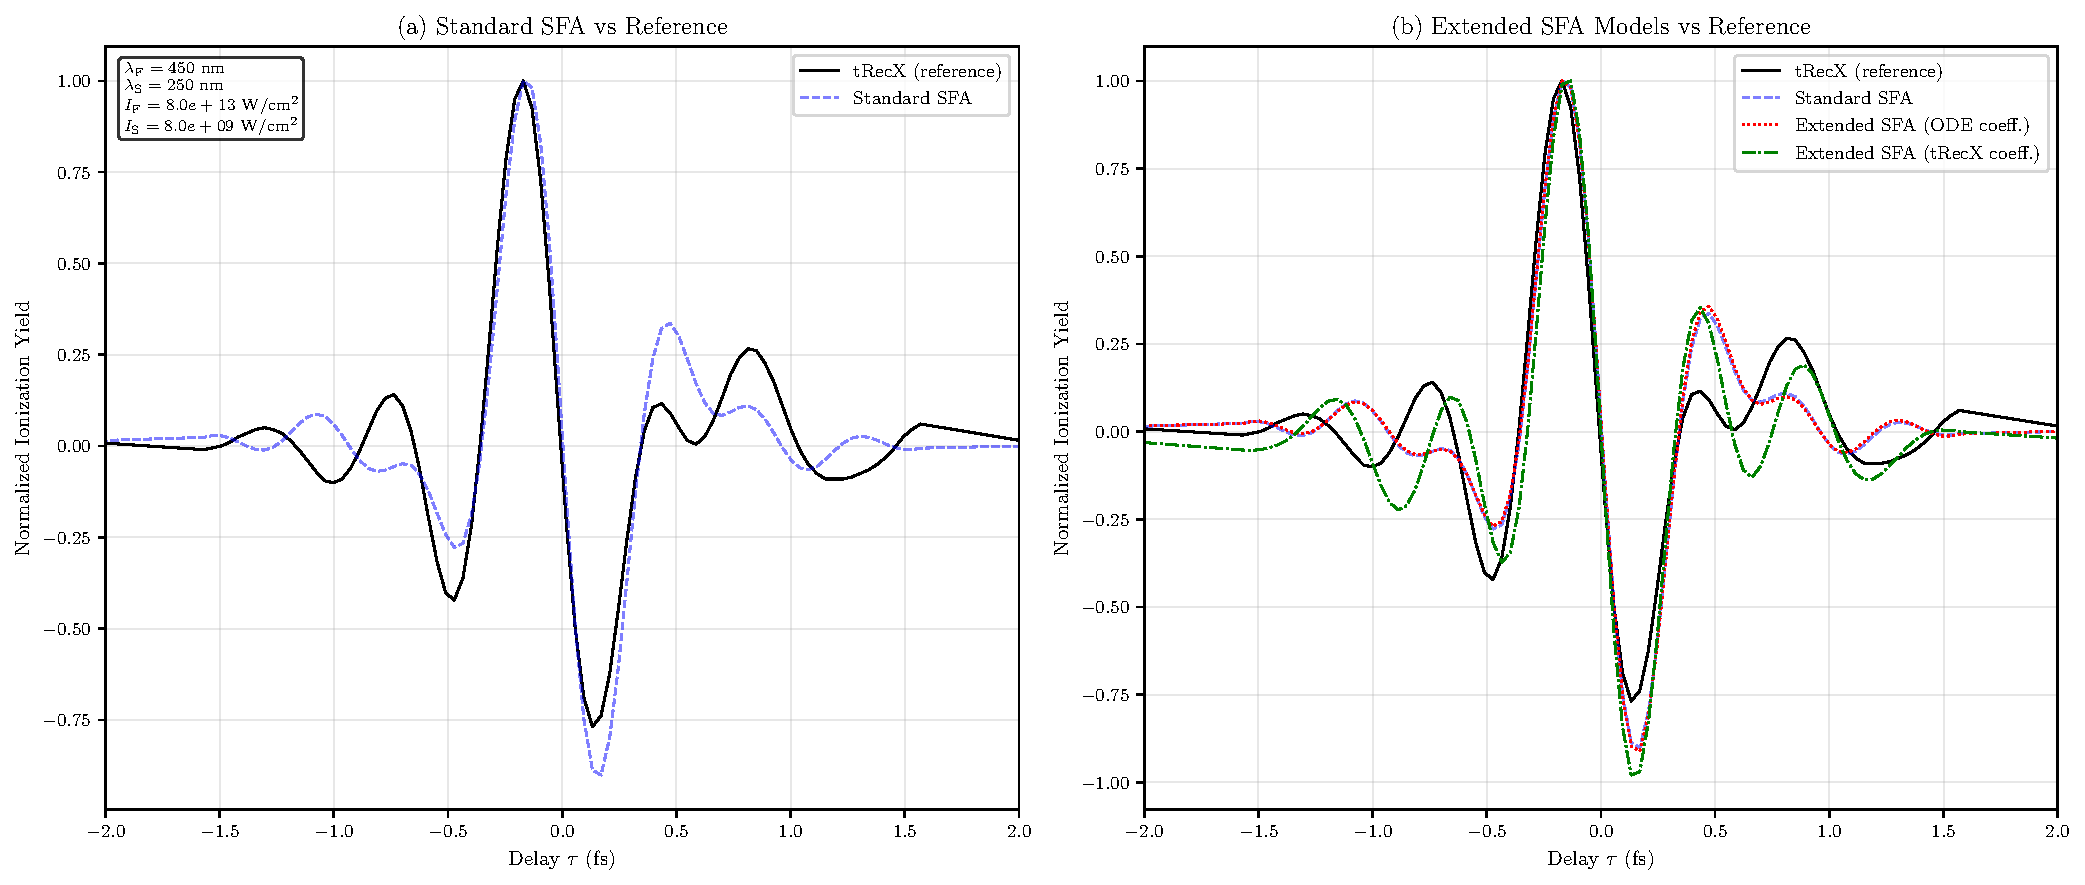
\includegraphics[width=1\textwidth]{../ionModel/python/plotsTIPTOE/2plot_SFA-comparison_1.pdf}
    \caption{Comparison of ionization yields from TIPTOE simulations between different SFA models and reference data from tRecX. 
            (a) Standart SFA overall does a good job reconstructing the ionization dynamics, but some parts it does not capture at all 
            (b) Extended SFA to excited states indeed shows some improvements in the reconstructing }
    \label{fig:tiptoe_sfa_comparison}
\end{figure}
Note that \eqref{eq:tiptoeprop} is fulfilled and it actually looks like the signal pulse.
On the left plot we see that tRecX is still orders of magnitude larger than the SFA results. 
However, with excited states it goes in the right direction as can be seen on the right plot. 
For three excited sates there is not much imporvement visible.
Unfortunately, the results are no where close to the tRecX measurements. That indicates that there is some physics missing in the SFA model.
If its not the excited states, the it must be something else.
And because the change is so big it has to be something more fundamental.
The first idea is that the interaction with the coulomb potential after ionization cannot be completely neglected, as it is done in the SFA model.
Even though it is counterintuitive, becasue if the coulomb potential is still noticable for the electron after ionization, why would it increase the results we are seeing??????
But this is in principle what our simulations are telling us. We can argue that we have two different ways of calculating the coefficients (ODE and tRecX) and the reproduce the same result.

However it indicates that real ionization propabilities do have some characterisitcs that the improved SFA model does not capture.

One also should make clear what the ODE coefficients do not capture. First, I implemented the code such that it ignores transitions not allowed by the dipole selection rules.

So in principle, assuming my SFA modification was correct the TIPTOE results tell us that the coulomb potential is not negligible after all. 
Maybe because the laser is not that intense (multiphoton ionization).
But its difficult to test that because if I increase the laser intensity, the approximations I made with the coefficients is not valid anymore.

Looking at not normalized results, tRecX is much more sensitive to the shift of probe and pump pulse, while excited SFA coefficients are not
Maybe because tRecX takes into account all the dynamics and effects inside an atom, while excited SFA coefficients does not care that much.
I would expect with tRecX coefficients more sensitive than with ODE coefficients???

\section{Influence of Stark Shift and Polarisation}
The Stark effect is the shift of the energy levels of an atom or molecule due to the presence of an external electric field.

\begin{figure}[H]
    \centering
    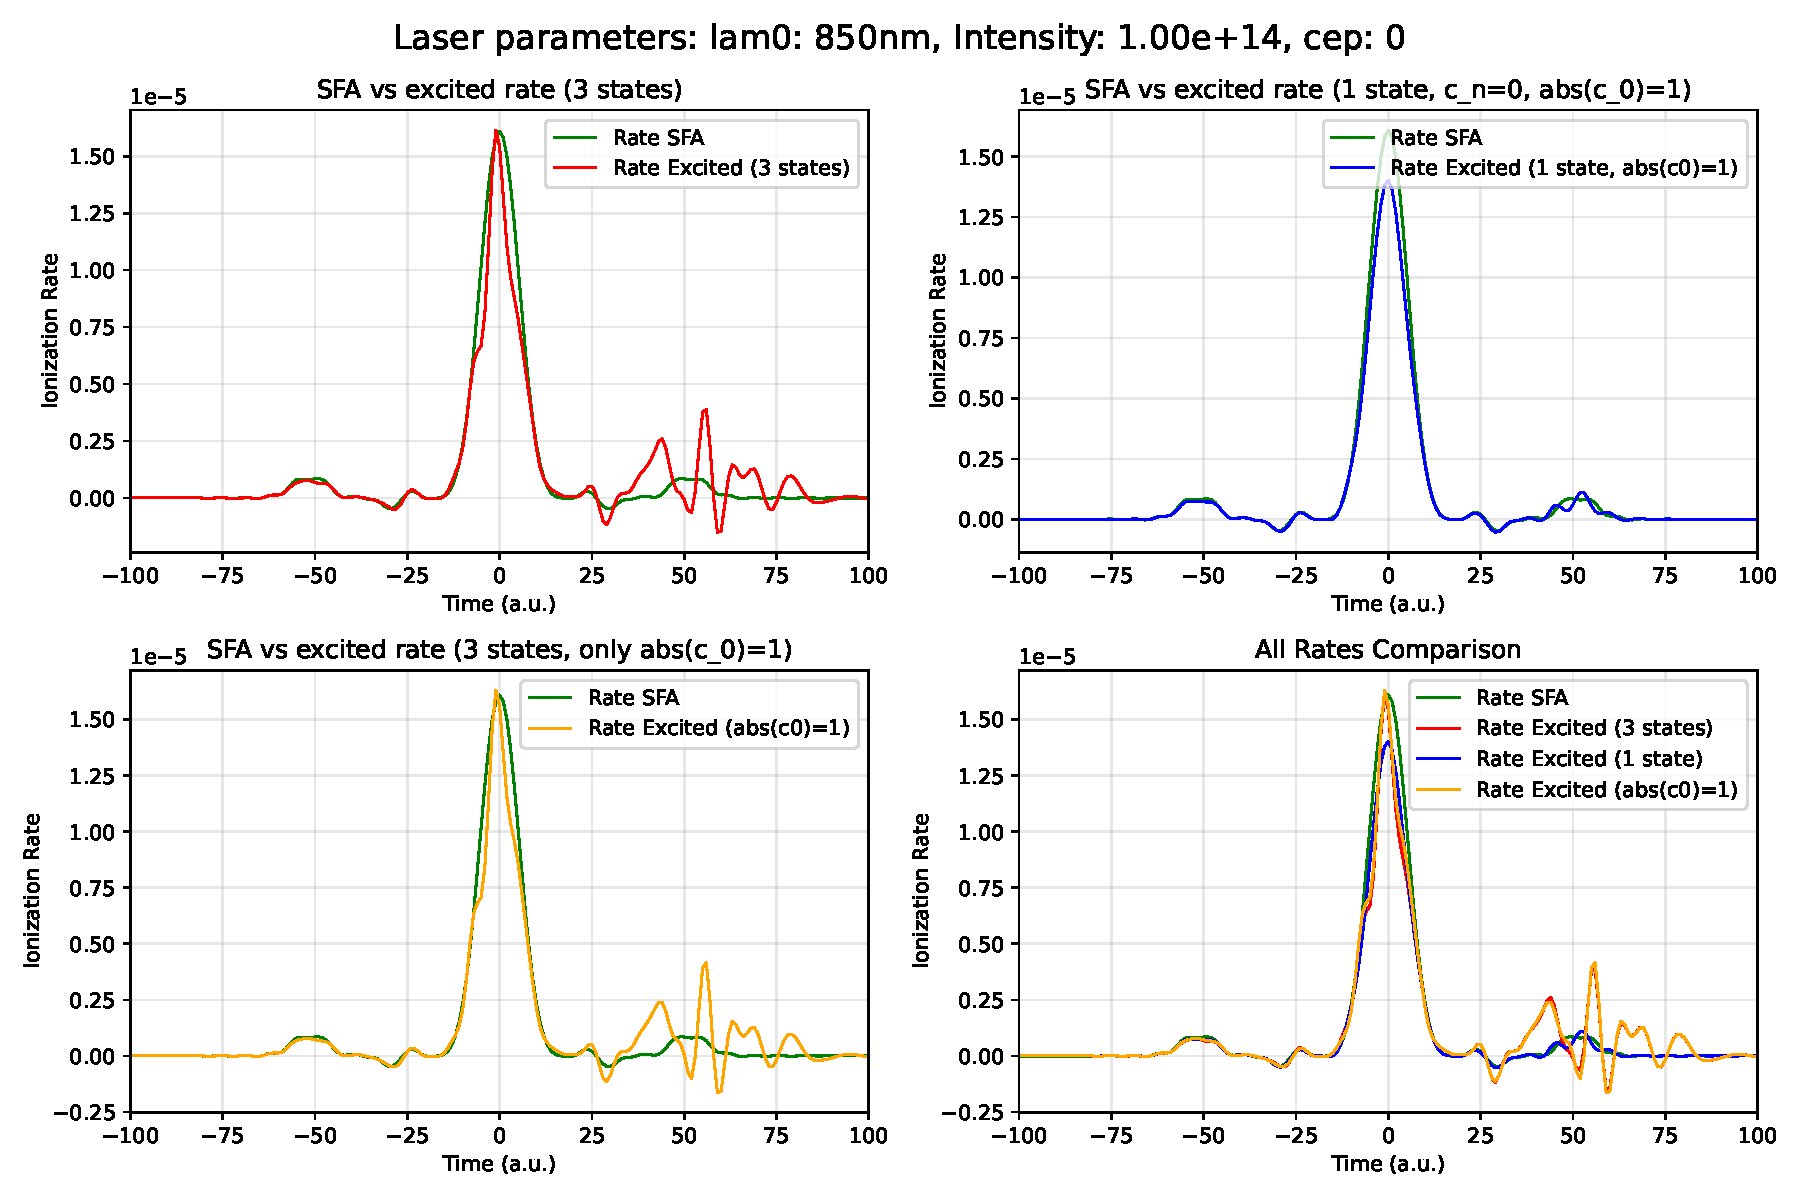
\includegraphics[width=0.9\textwidth]{figures/rate4_850_1.00e+14_onlystark.pdf}
    \caption{stark effect}
    \label{fig:starkeffect}
\end{figure}

Naiv: Stark effect changes energy in electron so its "harder" to ionise, thats why blue curve goes down (when excitedStates=1). 
But thats not certainly the case because of stark effect, thats why only set absc0 to 1 and phase remains. 
Example with oszillations with time dependent resonance frequency, and external force not at resonance but coincidence with oszillator resonance frequency so this may cause it.

\bigskip
Stark shift doesnt seem to have much contribution (sadly) but at least more than the polarisation of the ground state.

Lets investigate the influence of first coefficient, nothing more. Only the phase has a contribution, the amplitude is not important.
Thats because the amplitude determines something occupation propabilitiy, but the phase is $e^{-iEt}$ and if $E$ is shifted by a bit you can isolate it by just using purely the phase.\\
Top right is the isolated stark effect








% \section{Laser Fields}
% Lorem ipsum dolor sit amet, consetetur sadipscing elitr, sed diam nonumy eirmod tempor invidunt ut labore et dolore magna aliquyam erat, sed diam voluptua. At vero eos et accusam et justo duo dolores et ea rebum. Stet clita kasd gubergren, no sea takimata sanctus est Lorem ipsum dolor sit amet. Lorem ipsum dolor sit amet, consetetur sadipscing elitr, sed diam nonumy eirmod tempor invidunt ut labore et dolore magna aliquyam erat, sed diam voluptua. At vero eos et accusam et justo duo dolores et ea rebum. Stet clita kasd gubergren, no sea takimata sanctus est Lorem ipsum dolor sit amet.


% \begin{equation}
%     \partial_t u = \mathcal{H}(t)  \lambda 
% \end{equation}

% \begin{figure}[H]
%     \centering
%     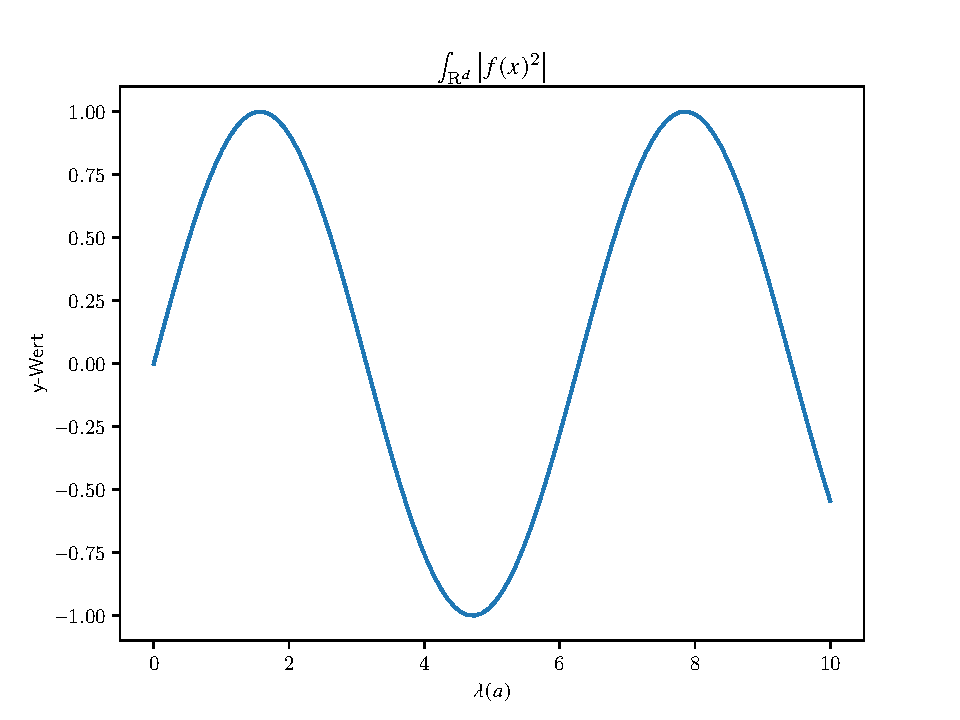
\includegraphics[width=0.5\textwidth]{figures/plot.pdf}
%     \caption{Sine function}
%     \label{fig:sinus}
% \end{figure}



% \begin{equation*}
%     \partial \A = \B
% \end{equation*}

% \medskip

% \begin{equation}
%     \int_{\R^d} \abs{f(x)}^2 \dd x = \int_{\R^d} \abs{\F f(\xi)}^2 \dd \xi
% \end{equation}

% \medskip

% \begin{equation}
%     %schrödinger equation
%     \ii \partial_t u = \mathcal{H}(t) \Ket{a} \lambda 
% \end{equation}

% \begin{equation}
%     \gimel \overrightarrow{a} \cos \mathrm{cos} \Rightarrow \Longrightarrow \nearrow 
% \end{equation}
